\section{Results}
\label{sec:results}

\paragraph{Setup.}
We evaluate $12$ (model $\times$ strategy) cells at $600$ scenarios $\times$ $3$ repeats.
A subprocess-isolated runner caught $62$ pathology scenarios in \structured\ cells (LLM-IR circular dependencies), keeping per-cell coverage $\geq 91\%$ except \geminiflash + \structured (blocked at the API layer; \cref{ssec:gemini_finding}); \opus + \structured ($574/600$) and \gpt + \structured ($545/600$) are marginally partial, marked $^*$ in \cref{tab:headline}.
The headline run uses the post-hardened verifier throughout (\cref{ssec:ver_defn}).

\begin{table}[t]
\caption{Headline leaderboard on the $600$-scenario $\times$ $3$-repeat draw (post-hardening). \textbf{T1/T2/T3} are strict pass-rates \emph{conditional on tier} (passes in tier $t$ / records in tier $t$ within the cell); \textbf{Strict} is the overall record-weighted rate over the cell. Tier rates do not column-average to \textbf{Strict} because per-tier record counts differ across cells (curriculum's T2-biased composition $36/128/37$ and marginal coverage on $^*$ cells). \textbf{Loose} $=$ \texttt{pass}$+$\texttt{soft\_pass}. Cells $^*$ are marginally partial; the $^\dagger$ cell is blocked at the API layer by Google's schema-state cap (\cref{ssec:gemini_finding}).}
\label{tab:headline}
\centering
\footnotesize
\setlength{\tabcolsep}{4pt}
\begin{tabular}{llrrrrrrrr}
\toprule
\textbf{Model} & \textbf{Strategy} & \textbf{N} & \textbf{T1} & \textbf{T2} & \textbf{T3} & \textbf{Strict} & \textbf{Loose} & \textbf{\$/scen.} & \textbf{Latency} \\
\midrule
\gpt & \structured & $2{,}304^*$ & 100\% & 100\% & 93\% & \textbf{94.1\%} & 94.1\% & \dollars{0.075} & 33.6\,s \\
\sonnet & \structured & $2{,}861$ & 100\% & 92\% & 87\% & 93.4\% & 93.4\% & \dollars{0.088} & 19.0\,s \\
\opus & \structured & $2{,}292^*$ & 100\% & 99\% & 82\% & 93.3\% & 93.3\% & \dollars{0.532} & 23.9\,s \\
\gpt & \rawcode & $1{,}800$ & 100\% & 91\% & 85\% & 91.9\% & 95.3\% & \dollars{0.058} & 14.8\,s \\
\geminipro & \structured & $1{,}140^{*}$ & 100\% & 92\% & --- & 83.1\% & 83.1\% & \dollars{0.050} & 75.7\,s \\
\sonnet & \rawcode & $1{,}800$ & 100\% & 73\% & 70\% & 81.2\% & 95.3\% & \dollars{0.044} & 16.4\,s \\
\haiku & \structured & $2{,}232$ & 89\% & 66\% & 74\% & 75.3\% & 76.8\% & \dollars{0.032} & 8.0\,s \\
\opus & \rawcode & $1{,}800$ & 98\% & 56\% & 61\% & 71.6\% & 95.3\% & \dollars{0.262} & 13.8\,s \\
\haiku & \rawcode & $2{,}403$ & 89\% & 60\% & 67\% & 70.5\% & 76.0\% & \dollars{0.019} & 9.5\,s \\
\geminipro & \rawcode & $1{,}800$ & 92\% & 38\% & 46\% & 58.4\% & 89.9\% & \dollars{0.049} & 32.9\,s \\
\geminiflash & \rawcode & $2{,}403$ & 33\% & 34\% & 41\% & 35.9\% & 42.2\% & \dollars{0.012} & 22.1\,s \\
\midrule
\geminiflash & \structured & $0^\dagger$ & --- & --- & --- & --- & --- & --- & --- \\
\bottomrule
\end{tabular}
\end{table}

\subsection{Two findings}
\label{ssec:findings}

\paragraph{Strategy choice helps unevenly.}
\structured\ lifts every model (\gpt + $2.2$\pp, \haiku + $4.8$, \sonnet + $12.2$, \opus + $21.7$, \geminipro + $24.7$): largest for the models weakest at \rawcode, smallest for the strongest.

\paragraph{Frontier convergence: three flagships tie within $1$\pp at \structured.}
\gpt, \sonnet, and \opus under \structured\ span only $0.8$\pp at a $\mathbf{7\times}$ cost ratio --- no measurable quality premium for the frontier-tier model under IR scaffolding.
At \rawcode, \gpt dominates \opus by $20$\pp at $4.5\times$ lower cost, and \haiku\ ties \opus at $14\times$ lower cost.

\subsection{Pareto and tier breakdown}
\label{ssec:pareto}

\begin{figure}[t]
\centering
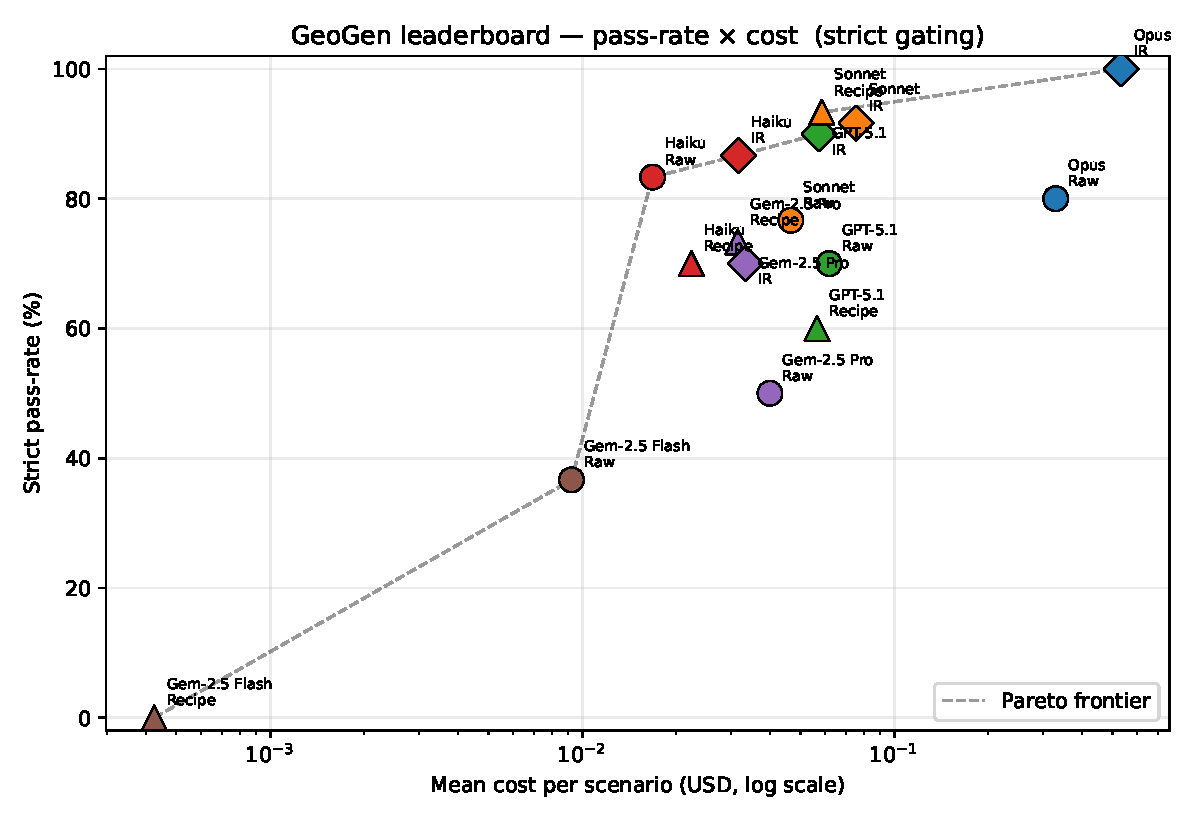
\includegraphics[width=0.6\linewidth]{figures/pareto.pdf}
\caption{Pareto frontier (cost vs strict pass, log-x) on the headline run. Seven of eleven cells are non-dominated.}
\label{fig:pareto}
\end{figure}

\gpt + \structured is the unique high-quality corner (\cref{fig:pareto}): it Pareto-dominates \sonnet + \structured ($+0.8$\pp at $17\%$ lower cost) and \opus + \structured ($+0.8$\pp at $7\times$ lower cost).
\opus + \rawcode is the most-dominated cell (\gpt + \rawcode beats it by $20$\pp at $4.5\times$ lower cost); \haiku + \rawcode is statistically tied with \opus + \rawcode at $14\times$ lower cost.
\geminiflash + \rawcode (\dollars{0.012}, $35.9$\%) is the price-floor frontier point; \geminipro + \structured (\dollars{0.050}, $83.1$\%) is on the frontier with caveat (\tthree\ throttled by Google's quota, so $83.1$\% is \tone--\ttwo only --- see Table~\ref{tab:headline}).
Reading the T1/T2/T3 columns in \cref{tab:headline}: \tone\ is near $100$\% for every Anthropic/OpenAI \structured\ cell (a signal that v2 needs harder \tone\ templates); \ttwo\ is where strategy first matters (\opus jumps $+43$\pp, $56\% \to 99\%$; \geminipro $+54$\pp, $38\% \to 92\%$); \tthree\ separates the three frontier+\structured\ cells (\gpt $93\%$, \sonnet $87\%$, \opus $82\%$).

\paragraph{Per-template heatmap and failure modes.}
The per-template heatmap (\cref{fig:heatmap}, \cref{app:template_specs}) exposes \textbf{universally easy} (every \tone\ template at or near $100$\% for each model's best strategy), \textbf{universally hard} (\texttt{tpl-t3-trv} at $\leq 16$\% for every cell), and \textbf{discriminating} templates (\texttt{tpl-t2-bis}, \texttt{tpl-t2-ic}, \texttt{tpl-t3-2alt}: model matters more than strategy).
The failure-mode breakdown (\cref{fig:failure_modes}, \cref{app:failure_coding}) shows failures dominated by geometric-predicate violations on the hardest templates: \propname{corresponding\_angles\_equal} alone accounts for $34$--$48$ failures per cell on \texttt{tpl-t3-trv}; \structured\ failures tilt toward timeout.
\emph{Most wrong outputs are rendered diagrams with the wrong geometry}, not broken LaTeX.

\subsection{Deployment finding: Gemini's schema-state cap}
\label{ssec:gemini_finding}

The \structured\ strategy depends on schema-constrained generation; OpenAI and Google compile the schema to a server-side FSM with vendor-specific caps.
Our \texttt{DiagramIR} schema (a discriminated union of 31 \texttt{DefStmt} variants) compiles to thousands of FSM states; OpenAI and \geminipro\ accommodate this, \geminiflash\ does not (HTTP 400 in 1.1--1.6\,s with \emph{``the specified schema produces a constraint that has too many states for serving''}).
This is not a capability gap (no token is generated); it is a cross-vendor portability concern for any benchmark shipping a multi-variant discriminated-union IR.
We report \geminiflash + \rawcode at $35.9$\% and exclude the blocked \structured cell.
Per-template case studies (\texttt{tpl-t3-trv} universal failure, \texttt{tpl-t3-tan} strategy discriminator with $-86$\pp \rawcode$\to$\structured gap on \opus, \texttt{tpl-t3-cen} self-referential pass) and the per-cell stability index (\gpt + \structured at $99.8\%$ all-same-verdict; the price-floor cells in the $30$--$70\%$ band) are in \cref{app:case_studies}.
